% =====================================================================
\chapter{Atención eficiente en memoria: caché KV, MQA, GQA y MLA}
\label{tema:2}
% =====================================================================

Al generar texto, un Transformer produce un token cada vez y reutiliza las claves y los valores de las posiciones anteriores. Esa reutilización ahorra cómputo, pero obliga a guardar y a leer en cada paso una caché que crece con la longitud del contexto y con el tamaño del lote, y que en contextos largos ocupa más memoria que los propios pesos. Este tema cuantifica esa caché, demuestra que con atención multicabeza la decodificación está necesariamente limitada por la memoria y estudia las tres variantes que la reducen: la atención multiconsulta (MQA), la atención de consultas agrupadas (GQA) y la atención latente multicabeza (MLA). Se sigue a Shazeer~\cite[§2.4 y §3]{mqa}, a Ainslie \emph{et al.}~\cite[§2]{gqa}, a DeepSeek-AI~\cite[§2.1]{deepseekv2} y la clase~10 de CS336~\cite{cs336}.

\section{La caché de claves y valores}

Sea una capa de atención con $H$ cabezas de dimensión $\dhd$. En la generación autorregresiva, al procesar el token $t$ se necesitan las consultas de $t$ y las claves y los valores de las posiciones $1,\dots,t$. Por la causalidad (módulo~14, tema~1), las claves y los valores de las posiciones $j<t$ no dependen de $t$: se calculan una vez y se guardan.

\begin{definicion}[Caché KV]\label{def:cache}
La \emph{caché KV} de una capa, tras procesar $T$ tokens, es el par de tensores $(K,V)$ con las claves y los valores de las $T$ posiciones para cada una de las $\nkv$ cabezas de clave y valor. Cada tensor tiene $T\cdot\nkv\cdot\dhd$ números por secuencia.
\end{definicion}

\begin{proposicion}[Tamaño de la caché KV]\label{prop:cache}
Un modelo de $L$ capas con $\nkv$ cabezas de clave y valor de dimensión $\dhd$, que procesa un lote de $b$ secuencias de $T$ tokens con $s$ bytes por número, necesita
\[
M_{\mathrm{KV}}=2\,L\,\nkv\,\dhd\,T\,b\,s\ \text{bytes}.
\]
\end{proposicion}

\begin{proof}
Por la \cref{def:cache}, cada capa guarda $T\nkv\dhd$ números para $K$ y otros tantos para $V$, por secuencia. Se multiplica por $2$ (claves y valores), por $L$ capas, por $b$ secuencias y por $s$ bytes.
\end{proof}

\begin{ejemplo}[Llama~2 70B]\label{ej:llama2kv}
Llama~2 70B tiene $L=80$, $H=64$ cabezas de consulta de dimensión $\dhd=128$ y usa GQA con $\nkv=8$~\cite{llama2}. En bf16 ($s=2$), por token y secuencia, la caché ocuparía $2\cdot 80\cdot 64\cdot 128\cdot 2=2\,621\,440$~bytes $=2{,}5$~MiB con atención multicabeza ($\nkv=64$) y ocupa $327\,680$~bytes $=320$~KiB con GQA. Para $T=4096$ y $b=16$, eso son $160$~GiB frente a $20$~GiB. Los pesos en bf16 ocupan unos $140$~GB.
\end{ejemplo}

\section{La decodificación está limitada por la memoria}

El módulo~17 definió la intensidad aritmética de una operación como el cociente entre FLOPs y bytes transferidos, y la comparó con la intensidad crítica del acelerador. El paso de atención de la decodificación tiene una intensidad que no mejora con el lote.

\begin{proposicion}[Intensidad de la atención en la decodificación]\label{prop:intensidad}
Sea una capa con $H$ cabezas de consulta y $\nkv$ cabezas de clave y valor de dimensión $\dhd$, y sea un paso de decodificación de una secuencia cuyo contexto tiene $T$ posiciones. Contando solo los productos $q\,K\T$ y $a\,V$ y la lectura de la caché, la intensidad aritmética es
\[
I=\frac{2H}{s\,\nkv}\ \text{FLOP/byte},
\]
independiente de $T$ y del tamaño del lote. Con MHA ($\nkv=H$) en bf16, $I=1$.
\end{proposicion}

\begin{proof}
Para cada cabeza de consulta, el producto de $q\in\R^{1\times\dhd}$ por $K\T\in\R^{\dhd\times T}$ cuesta $2\dhd T$ FLOPs, y el de los pesos $a\in\R^{1\times T}$ por $V\in\R^{T\times\dhd}$, otros $2T\dhd$. Con $H$ cabezas: $F=4HT\dhd$. Los bytes leídos de la caché son $Q=2T\nkv\dhd s$, porque cada cabeza de clave y valor se lee una vez y la comparten las $H/\nkv$ consultas de su grupo. Entonces $I=F/Q=4HT\dhd/(2T\nkv\dhd s)=2H/(s\nkv)$. Con un lote de $b$ secuencias, $F$ y $Q$ se multiplican por $b$, porque cada secuencia tiene su propia caché, y el cociente no cambia.
\end{proof}

La intensidad crítica de la A100 en bf16 es $\Icrit\approx 156$~FLOP/byte (módulo~17, tema~2). Con MHA, la atención de la decodificación aprovecha menos del $1\,\%$ del cómputo disponible, y aumentar el lote no ayuda. Los productos de las matrices de pesos, en cambio, sí ganan intensidad con el lote, porque todas las secuencias comparten los mismos pesos. Shazeer llega a la misma conclusión con otro recuento: en la decodificación incremental con MHA, el cociente entre accesos a memoria y operaciones es $\Theta(n/d+1/b)$, y el término $n/d$, debido a la lectura de las claves y los valores, no disminuye con el lote~\cite[§2.4.1]{mqa}. Reducir $\nkv$ es la forma directa de atacarlo.

\section{Atención multiconsulta y de consultas agrupadas}

\begin{definicion}[MQA y GQA]\label{def:gqa}
Sea $H$ divisible por $G$. La \emph{atención de consultas agrupadas} con $G$ grupos (GQA-$G$) divide las $H$ cabezas de consulta en $G$ grupos de $H/G$ cabezas consecutivas; todas las cabezas de un grupo comparten una única cabeza de clave y una de valor~\cite[§2.2]{gqa}. Con proyecciones $W_Q^{(i)}\in\R^{d\times\dhd}$ para $i=1,\dots,H$ y $W_K^{(g)},W_V^{(g)}\in\R^{d\times\dhd}$ para $g=1,\dots,G$, la cabeza $i$ usa la clave y el valor del grupo $g(i)=\lceil iG/H\rceil$. El caso $G=1$ es la \emph{atención multiconsulta} (MQA)~\cite[§3]{mqa}, y el caso $G=H$ es la atención multicabeza.
\end{definicion}

\begin{proposicion}[Ahorro de GQA]\label{prop:gqa}
Con $\nkv=G$, respecto de MHA:
\begin{enumerate}
  \item la caché KV se divide exactamente por $H/G$;
  \item las proyecciones de clave y valor pasan de $2d^{2}$ a $2d\,G\dhd$ parámetros, y las de consulta y salida no cambian;
  \item la intensidad de la \cref{prop:intensidad} se multiplica por $H/G$.
\end{enumerate}
\end{proposicion}

\begin{proof}
(i) y (iii) se siguen de sustituir $\nkv=G$ en las \cref{prop:cache,prop:intensidad}. (ii) Con MHA hay $H$ proyecciones $d\times\dhd$ para $K$ y otras tantas para $V$, es decir, $2Hd\dhd=2d^{2}$ parámetros si $H\dhd=d$; con GQA hay $G$ de cada tipo, $2Gd\dhd$. Las consultas siguen teniendo $H$ cabezas y $W_O$ sigue siendo $d\times d$.
\end{proof}

\begin{figure}[ht]
\centering
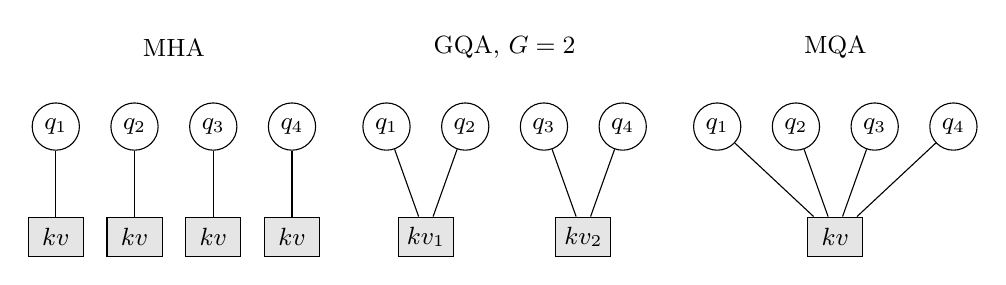
\begin{tikzpicture}[font=\small,q/.style={draw,circle,minimum size=6mm,inner sep=0pt},kv/.style={draw,rectangle,fill=black!10,minimum width=7mm,minimum height=5mm,inner sep=0pt}]
  \foreach \x/\lab in {0/MHA, 4.2/{GQA, $G=2$}, 8.4/MQA}{\node at (\x+1.5,2.4) {\lab};}
  % MHA
  \foreach \i in {0,1,2,3}{\node[q] (a\i) at (\i,1.4) {$q_{\the\numexpr\i+1}$}; \node[kv] (ak\i) at (\i,0) {$kv$}; \draw (a\i)--(ak\i);}
  % GQA
  \foreach \i in {0,1,2,3}{\node[q] (b\i) at (4.2+\i,1.4) {$q_{\the\numexpr\i+1}$};}
  \node[kv] (bk0) at (4.7,0) {$kv_1$}; \node[kv] (bk1) at (6.7,0) {$kv_2$};
  \draw (b0)--(bk0) (b1)--(bk0) (b2)--(bk1) (b3)--(bk1);
  % MQA
  \foreach \i in {0,1,2,3}{\node[q] (c\i) at (8.4+\i,1.4) {$q_{\the\numexpr\i+1}$};}
  \node[kv] (ck) at (9.9,0) {$kv$};
  \foreach \i in {0,1,2,3}{\draw (c\i)--(ck);}
\end{tikzpicture}
\caption{Cabezas de consulta y cabezas de clave y valor en MHA, GQA con dos grupos y MQA, con $H=4$.}
\label{fig:gqa}
\end{figure}

Shazeer observó que MQA reduce el tiempo de decodificación por token de 46 a 3,8~microsegundos en su experimento de traducción, con una pérdida de calidad pequeña pero apreciable~\cite[§4.2 y §4.3]{mqa}. Ainslie \emph{et al.} proponen GQA como término medio y muestran, además, que un modelo entrenado con MHA puede convertirse en uno con GQA sin entrenarlo desde cero: se promedian las proyecciones de clave y valor de las cabezas de cada grupo y se continúa el entrenamiento durante un $5\,\%$ de los pasos originales (\emph{uptraining})~\cite[§2.1 y §3.1]{gqa}. GQA con 8 grupos queda cerca de MHA en calidad y cerca de MQA en velocidad. Llama~2 la usa en sus modelos de 34B y 70B~\cite[tabla~1]{llama2}, y Llama~3, Mixtral y Grok-1 en todos sus tamaños (\cref{tab:hiper}).

\begin{ejemplo}[Grok-1]\label{ej:grokkv}
Grok-1 tiene $L=64$, $H=48$ cabezas de consulta y $\nkv=8$, con $\dhd=128$ y contexto máximo de 8192 tokens~\cite{grok1}. Por la \cref{prop:cache}, en bf16 la caché de una secuencia completa ocupa $2\cdot 64\cdot 8\cdot 128\cdot 8192\cdot 2=2^{31}$~bytes $=2$~GiB; con MHA serían $48/8=6$ veces más, $12$~GiB.
\end{ejemplo}

\section{Atención latente multicabeza}

GQA reduce la caché eliminando cabezas de clave y valor. MLA, introducida en DeepSeek-V2, conserva $H$ cabezas, pero guarda en la caché un único vector de baja dimensión por token del que se reconstruyen todas las claves y todos los valores~\cite[§2.1.2]{deepseekv2}.

\begin{definicion}[MLA sin codificación de posición]\label{def:mla}
Sean $\dc\ll H\dhd$, $W^{DKV}\in\R^{d\times\dc}$ y, para cada cabeza $i$, $W^{UK}_i,W^{UV}_i\in\R^{\dc\times\dhd}$ y $W^{Q}_i\in\R^{d\times\dhd}$. Para el token $t$ con entrada $h_t\in\R^{1\times d}$,
\[
c_t=h_tW^{DKV}\in\R^{1\times\dc},\qquad k_{t,i}=c_tW^{UK}_i,\qquad v_{t,i}=c_tW^{UV}_i,\qquad q_{t,i}=h_tW^{Q}_i .
\]
La caché guarda solo los vectores latentes $c_1,\dots,c_T$.
\end{definicion}

Guardar $c_t$ en lugar de $k_{t,i}$ y $v_{t,i}$ solo ahorra memoria si no hay que reconstruir explícitamente las claves y los valores en cada paso. La factorización lo evita.

\begin{proposicion}[Absorción de las proyecciones]\label{prop:absorcion}
Con la notación de la \cref{def:mla}, sean $\tilde q_{t,i}=q_{t,i}(W^{UK}_i)\T\in\R^{1\times\dc}$ y $a_{t,i,j}$ los pesos de atención de la cabeza $i$. Entonces
\[
q_{t,i}\,k_{j,i}\T=\tilde q_{t,i}\,c_j\T,\qquad \sum_{j\le t}a_{t,i,j}\,v_{j,i}=\Bigl(\sum_{j\le t}a_{t,i,j}\,c_j\Bigr)W^{UV}_i .
\]
En consecuencia, las puntuaciones y la salida de cada cabeza se calculan a partir de los $c_j$, sin formar $k_{j,i}$ ni $v_{j,i}$; además, $W^{UK}_i$ puede integrarse en la proyección de consulta y $W^{UV}_i$, en la de salida.
\end{proposicion}

\begin{proof}
$q_{t,i}k_{j,i}\T=q_{t,i}(c_jW^{UK}_i)\T=q_{t,i}(W^{UK}_i)\T c_j\T=\tilde q_{t,i}c_j\T$, por la regla de la traspuesta de un producto. Para la segunda igualdad, $\sum_j a_{t,i,j}c_jW^{UV}_i=(\sum_j a_{t,i,j}c_j)W^{UV}_i$ por la distributividad del producto de matrices. Por último, $\tilde q_{t,i}=h_t\bigl(W^{Q}_i(W^{UK}_i)\T\bigr)$, con $W^{Q}_i(W^{UK}_i)\T\in\R^{d\times\dc}$ fija, y la salida de la cabeza se multiplica después por el bloque $i$ de $W_O$, de modo que $W^{UV}_iW_O^{(i)}$ es también una matriz fija.
\end{proof}

\begin{observacion}[RoPE desacoplada]
La absorción falla con RoPE. Con vectores fila, la rotación de la posición $m$ actúa como $x\mapsto xR_m$, y $R_mR_n\T=R_{m-n}$ (es la versión traspuesta de la identidad del módulo~14, tema~4). Si la consulta y la clave se rotan, la puntuación es $q_{t,i}R_t(c_jW^{UK}_iR_j)\T=q_{t,i}R_{t-j}(W^{UK}_i)\T c_j\T$: entre $q_{t,i}$ y $c_j$ aparece una matriz que depende de la distancia $t-j$, y ya no hay una matriz fija que integrar en la consulta. DeepSeek-V2 lo resuelve añadiendo a cada cabeza una componente de dimensión $d_h^{R}$ que sí se rota y cuya clave $k^{R}_t$ es compartida por todas las cabezas y se guarda también en la caché~\cite[§2.1.3]{deepseekv2}. La caché por token y capa tiene entonces $\dc+d_h^{R}$ números.
\end{observacion}

\begin{table}[ht]
\centering\small
\caption{Números guardados en la caché KV por token, en un modelo de $L$ capas~\cite[tabla~1]{deepseekv2}.}\label{tab:mla}
\begin{tabular}{@{}lll@{}}
\toprule
Mecanismo & Caché por token & DeepSeek-V2 ($L=60$, $H=\dhd=128$) \\
\midrule
MHA & $2H\dhd L$ & $1\,966\,080$ \\
GQA-$G$ & $2G\dhd L$ & $15\,360\,G$ \\
MQA & $2\dhd L$ & $15\,360$ \\
MLA & $(\dc+d_h^{R})L$ & $(512+64)\cdot 60=34\,560$ \\
\bottomrule
\end{tabular}
\end{table}

\begin{ejemplo}[DeepSeek-V2]\label{ej:mla}
DeepSeek-V2 usa $L=60$, $H=128$, $\dhd=128$, $\dc=512=4\dhd$ y $d_h^{R}=64=\dhd/2$~\cite{deepseekv2}. La caché por token tiene $(\dc+d_h^{R})L=\frac92\dhd L=34\,560$ números, frente a $1\,966\,080$ con MHA: $56{,}89$ veces menos. Equivale a la caché de GQA con $576/(2\cdot 128)=2{,}25$ grupos. En bf16 son $69\,120$~bytes $=67{,}5$~KiB por token; un contexto de $2^{17}=131\,072$ tokens ocupa $8{,}44$~GiB, frente a $480$~GiB con MHA. Según el artículo, MLA supera a MHA en calidad en sus experimentos y reduce la caché un $93{,}3\,\%$ respecto de su modelo denso anterior~\cite{deepseekv2}.
\end{ejemplo}

\begin{lecturas}
\item Shazeer~\cite{mqa}, §2.4 «Multihead Attention (Incremental)» y §3 «Multi-Query Attention».
\item Ainslie \emph{et al.}~\cite{gqa}, §2.1 «Uptraining» y §2.2 «Grouped-query attention».
\item DeepSeek-AI~\cite{deepseekv2}, §2.1 «Multi-Head Latent Attention», con la tabla~1.
\item Stanford CS336~\cite{cs336}, clase~10, «Inference»: reducción de la caché KV (GQA, MLA, atención entre capas y atención local).
\item Temario de CMU 11-868~\cite{cmu11868}: sistemas de inferencia y servicio de modelos.
\end{lecturas}

\section*{Ejercicios del tema 2}
\addcontentsline{toc}{section}{Ejercicios del tema 2}

\begin{ejercicio}{1}{eje:2-vf}
Justifique si son verdaderas o falsas: (a) GQA reduce los FLOPs de la proyección de consulta; (b) con MQA, la caché KV por token y capa no depende del número de cabezas de consulta; (c) MLA guarda en la caché las claves y los valores de cada cabeza en una dimensión reducida.
\end{ejercicio}

\begin{ejercicio}{2}{eje:2-kv}
Un modelo tiene 32 capas, 32 cabezas de consulta con $\dhd=128$ y trabaja en bf16. Calcule la caché KV de una secuencia de $T=8192$ tokens con MHA, con GQA-8 y con MQA, en las unidades binarias más adecuadas.
\end{ejercicio}

\begin{ejercicio}{2}{eje:2-cs336}
Sea un modelo con la forma de Llama~2 13B: $V=32\,000$, $d=5120$, $\dff=13\,824$, $L=40$ y 40 cabezas de consulta con $\dhd=128$. Se sirve en bf16 con secuencias de $T=1024$ tokens, en un acelerador con ancho de banda de memoria de $3{,}35$~TB/s, y se supone que cada paso de decodificación lee una vez todos los pesos y toda la caché. Para (a) MHA ($\nkv=40$) y (b) GQA con $\nkv=8$, ambos con lote $b=64$, calcule los parámetros, la memoria total, la latencia por paso y el rendimiento en tokens por segundo.
\fuente{adaptado de Stanford CS336~\cite{cs336}, clase~10 («Inference»), ejemplo de Llama~2 13B con caché reducida mediante GQA.}
\end{ejercicio}

\begin{ejercicio}{2}{eje:2-intens}
Con la \cref{prop:intensidad}, calcule la intensidad aritmética de la atención en la decodificación de Llama~2 70B en bf16, con MHA, con su GQA-8 y con MQA. Compare cada valor con $\Icrit\approx 156$~FLOP/byte y calcule qué fracción del rendimiento máximo de la A100 se alcanza según el modelo \emph{roofline}.
\end{ejercicio}

\begin{ejercicio}{2}{eje:2-mla}
Un modelo hipotético con MLA tiene $L=40$, $H=32$, $\dhd=128$, $\dc=256$ y $d_h^{R}=64$. (a) Calcule la caché por token con MLA y con MHA, en número de valores y en bytes (bf16). (b) ¿A cuántos grupos de GQA equivale? (c) ¿Cuántos tokens de contexto caben en 16~GiB de caché con cada mecanismo?
\end{ejercicio}

\begin{ejercicio}{3}{eje:2-pool}
Sea un modelo MHA en el que, dentro de cada grupo de $H/G$ cabezas, todas las proyecciones de clave coinciden entre sí y lo mismo ocurre con las de valor. (a) Demuestre que su conversión a GQA-$G$ promediando las proyecciones de cada grupo produce exactamente las mismas salidas. (b) Muestre con un ejemplo de dos cabezas con $\dhd=1$ que, si las proyecciones no coinciden, las puntuaciones cambian en general.
\end{ejercicio}

\begin{ejercicio}{3}{eje:2-rope}
Con la notación de la \cref{def:mla} y vectores fila, suponga que la clave se rota, $k_{j,i}=c_jW^{UK}_iR_j$, y la consulta, $q_{t,i}R_t$, donde $R_m$ es la matriz ortogonal de RoPE en la posición $m$ y $R_m R_n\T=R_{m-n}$. (a) Escriba la puntuación $q_{t,i}R_t(c_jW^{UK}_iR_j)\T$ como $q_{t,i}\,M_{t,j}\,c_j\T$ e identifique $M_{t,j}$. (b) Suponiendo que todas las frecuencias de RoPE cumplen $0<\theta_l<2\pi$, demuestre que $M_{t,j}$ toma el mismo valor para todos los pares $(t,j)$ solo si $W^{UK}_i=0$, y explique por qué esto impide la absorción.
\end{ejercicio}
